\documentclass[12pt]{beamer}
\usepackage{graphicx}
\usetheme{Amsterdam}

\title{Mapreduce Simple Tutorial \& Homework}
\author{Wen-Chieh Wu}
\date{May 18, 2014}

\begin{document}

\maketitle

\begin{frame}
  \frametitle{HDFS}
  Hadoop Distributed File System : Designed to reliably store very large files across machines in a large cluster
  \begin{itemize}
    {\item hadoop fs -ls}\\
      List files in the /user/[your account name]\\
      ex: /user/r01922003
    {\item hadoop fs -mkdir [dir]}\\
      Create folder in the /user/[your account name]/[dir]
    {\item hadoop fs -rm -r [dir]}\\
      Delete folder /user/[your account name]/[dir]
  \end{itemize}
\end{frame}

\begin{frame}
  \frametitle{HDFS(cont.)}
  \begin{itemize}
    {\item hadoop fs -put [localfile] [dir]/[file]}\\
      Push files [localfile] to /user/[your account name]/[dir]/[file]
    {\item hadoop fs -get [dir]/[file] [localfile]}\\
      Get files from /user/[your account name]/[dir]/[file] to [localfile]
    {\item hadoop fs -getmerge [dir] [localfile]}\\
      From [dir], get the merged result
  \end{itemize}
\end{frame}

\begin{frame}
  \frametitle{MapReduce}
  Programming model for processing large data sets with a parallel, distributed algorithm on a cluster.\\
  Written in Java, usually we divided to three .java files, take wordcount as an example\\
  \begin{itemize}
    {\item WordCount.java}
    {\item WordCountMapper.java}
    {\item WordCountReducer.java}
  \end{itemize}
\end{frame}

\begin{frame}
  \frametitle{MapReduce(cont.)}
  \begin{block}{How to compile? shortcut: \$ make}
    \$ javac -classpath `yarn classpath` WordCount.java WordCountMapper.java WordCountReducer.java\\
    \$ jar -cvf WordCount.jar WordCount.class WordCountMapper.class WordCountReducer.class\\
  \end{block}

  \begin{block}{How to execute? shortcut: \$ make run}
    \$ hadoop jar WordCount.jar WordCount inputdir outputdir
  \end{block}

  \begin{block}{How to know the result? shortcut: \$ make get}
    \$ hadoop fs -getmerge outputdir result\\
    \$ cat result
  \end{block}
\end{frame}

\begin{frame}
  \frametitle{MapReduce(cont.)}
  Notes
  \begin{itemize}
    {\item The cluster executes one application a time, you need to wait for it.}
    {\item Jobtracker: http://140.112.2.92:8088/}
  \end{itemize}
\end{frame}


\begin{frame}
  \frametitle{Examples}
  \begin{itemize}
    {\item helloworld}\\
      Output Hello World message
    {\item stringsort}\\
      Sort files of strings
    {\item wordcount}\\
      Classic example that calculate the word count of files
  \end{itemize}
\end{frame}

\begin{frame}
  \frametitle{Examples(cont.)}
  \begin{center}
    {\Large Let's take a look at the examples}\\
    {\Large \$ cp -r /tmp/mapreduce.example .}
  \end{center}
\end{frame}

\begin{frame}
  \frametitle{Homework}
  \begin{center}
    {\Large Use mapreduce to sort file size for files,\\ from min. to max.}
  \end{center}
\end{frame}

\begin{frame}
  \frametitle{Homework(cont.)}
  The problem can be regarded as a file size sorting problem, the first column is the file size and the latter column is the file name.
  \begin{block}{Input}
    \begin{tabular}{ll}
      100 & apple\\
      33  & orange\\
      100 & banana \\
      10 & pineapple\\
    \end{tabular}
  \end{block}

  \begin{block}{Output}
    \begin{tabular}{ll}
      10 & pineapple\\
      33  & orange\\
      100 & apple,banana \\
    \end{tabular}
  \end{block}
\end{frame}

\begin{frame}
  \frametitle{Homework(cont.)}
  There are four dataset
  \begin{itemize}
    {\item /data/easy, 16 sec}
    {\item /data/tiny, 21 sec}
    {\item /data/small, 1 min 19 sec}
    {\item /data/big, 12 min 9 sec}
  \end{itemize}
\end{frame}

\begin{frame}
  \frametitle{Homework(cont.)}
  Requirement
  \begin{itemize}
    {\item Processing 4 dataset without error, output format is right and each part is sorted by file size.(70\%)}
    {\item The file name is sorted by alphabet.(15\%)}
    {\item The ``-getmerge'' result is sorted by file size.(15\%)}
  \end{itemize}
\end{frame}

\begin{frame}
  \frametitle{Homework(cont.)}
  Hints
  \begin{itemize}
    {\item The range of the file size is between 0 and 2147483647.}
    {\item There are five reducers only.}
    {\item Please research ``MapReduce Partitioner'', it will be useful for the requirement 3.}
    {\item We will provide ``IteratorSort.java'', it can help you sort the file names.}
  \end{itemize}
\end{frame}

\begin{frame}
  \frametitle{Homework(cont.)}
  IteratorSort.java Usage, remember to compile it with other .java files
  \begin{center}
    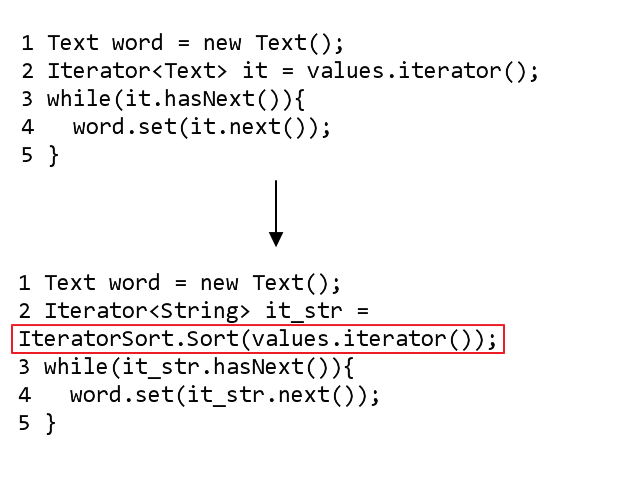
\includegraphics[scale=0.4]{img/code.png}
  \end{center}
\end{frame}

\begin{frame}
  \frametitle{Homework(cont.)}
  In the zip file
  \begin{itemize}
    {\item pdp.hw3.mapreduce.pdf}
    {\item IteratorSort.java}
    {\item easy.ans}
    {\item tiny.ans}
  \end{itemize}
  you can use ``diff'' to check the answer
\end{frame}

\begin{frame}
  \frametitle{Homework(cont.)}
  Please upload your program to CEIBA, in the zip file contain a folder of your id and the program *.java, a readme.txt telling me how to compile \& execute the program.\\
  EX:\\
  \begin{itemize}
    {\item r01922003}
          \begin{itemize}
            {\item *.java}
            {\item readme.txt}
          \end{itemize}
  \end{itemize}
\end{frame}

\begin{frame}
  \frametitle{Homework(cont.)}
  Grading
  \begin{itemize}
    {\item Deadline: 6/4 14:00}
    {\item 10\% off for late submission each week, latest submission date: 6/25}
    {\item If your program executes for too long, you may lose some grades.}
  \end{itemize}
\end{frame}

\end{document}
